\documentclass{article}
\usepackage[utf8]{inputenc}
\usepackage{fancyhdr}
\usepackage[margin=2.8cm,twoside]{geometry}
\usepackage[super]{nth}
\usepackage[english]{babel}
\usepackage{csquotes}

\usepackage{hyperref}
\usepackage[backend=biber,style=ieee]{biblatex}
\addbibresource{bibliography.bib}

\usepackage{float}

\pagestyle{fancy}
\fancyhf{}
\fancyhead[LE,RO]{DID - 04 Preliminary Design (Hebb \& Stephan)}
\fancyhead[LO,RE]{\leftmark}
\fancyfoot[LE,RO]{\thepage}

\usepackage{graphicx}

\begin{document}
	
\begin{titlepage}
	\begin{center}
		\vspace*{1cm}
		
		\LARGE\textsc{Royal Military College of Canada}\normalsize
		
		\vspace{0.2cm}
		
		\textsc{Department of Electrical and Computer Engineering}
		
		\vspace{1.5cm}
		
		
\includegraphics[width=0.3\textwidth]{rmcLogo.png}
		
		\vspace{1.5cm}
		
		\LARGE{Designing Coatimunde\\}
		
		\vspace{0.2cm}
		
		\normalsize{Computer Optics Analyzing Trajectories In Mostly Unknown, Navigation Denied, Environments}
		
		\vspace{0.1cm}
		
		\normalsize{DID-04 - Preliminary Design}
		
		\vfill
		
		\textbf{Presented by:}\\Amos Navarre \textsc{Hebb} \& Kara \textsc{Stephan}\\
		\vspace{0.8cm}
		\textbf{Presented to:}\\Dr. Sidney \textsc{Givigi} \& Dr. Rachid \textsc{Beguenane}
		\vspace{0.8cm}
		
		\today
		
	\end{center}
\end{titlepage}

% \begin{abstract}
% \end{abstract}


\tableofcontents

\newpage

\section{Introduction}

	\subsection{Document Purpose}
	
	Using Computer Optics for Analyzing Trajectories in Mostly Unknown, Navigation Denied, Environments (\textsc{coatimunde}) is the goal of this project. The purpose of this document is to outline the preliminary design for \textsc{coatimunde}. That is, what the design of the project is, how it will be built, and how this meets the requirements for the project. These requirements have been outlined in the Statement of Requirements. The design of the project thus far will be shown and discussed within the Design Section. This document will then identify the constraints, risks, and difficulties that have been faced so far in the project.
	
	\subsection{Background}
	
	Both in the consumer and professional sectors the use of autonomous aerial vehicles is growing quickly. Currently these vehicles rely on skilled pilots to accomplish a very limited set of tasks. Adding obstacle avoidance capabilities to these vehicles and simplifying the task of following targets could allow for these systems to be used in many more situations. This section will give a quick background on obstacle avoidance, unmanned aircraft systems, computer vision, and the platforms we intend to use in this project.
	
		\subsubsection{Obstacle Avoidance}
		
		
		Obstacle avoidance is the task of satisfying a control objective, in this case moving toward a visual target, while subject to non-intersection or non-collision position constraints. The latter constraints are, in this case, to be dynamically created while moving in a reactive manner, instead of being pre-computed.
		
		\subsubsection{Unmanned Aircraft Systems}
		
		Very generally any powered vehicle that uses aerodynamic forces to provide lift, without a human operator being carried, can be considered an unmanned aerial vehicle. Currently most of these vehicles make up a single component of a larger unmanned aircraft system. 
		
		An Unmanned aircraft system (UAS), or remotely piloted aircraft system (RPAS), is an aircraft without a human pilot on-board, instead controlled from an operator on the ground. Such a system can have varying levels of autonomy, something as simple as a model aircraft could be considered a UAS without any automation capabilities. Detecting, recognizing, identifying, and tracking targets of interest in complex environments and integrate with the systems required to process and fuse the collected information into actionable intelligence while operating in a low-to-medium threat environment is the current goal of the RPAS project by the Royal Canadian Air Force (RCAF) \cite{RPAS}. 
		
		Flying a UAS requires a secure link to the operator off-board. Maintaining this link, particularly while flying close to the ground where more opportunities for interference are introduced is difficult. This difficulty is compounded in environments where potentially hostile actors may be attempting to jam communications. This necessitates a level of automation on-board capable of maintaining flight while denied navigation information.
		
		There are many different types of approaches for this problem, but most involve some form of identifying targets in real time and reacting as they become visible to the aircraft. This has proven successful on a flying robot traveling at high speeds \cite{barry2015pushbroom}. This system successfully combined trajectory libraries and a state machine to avoid obstacles using very little computational power even at very high speeds \cite{barry2018high}. Another solution to obstacle avoidance on flying robots was the creation of NanoMap \cite{2018nanomap}. This allows for 3D data to be processed at a much faster rate allowing for higher speeds of the robot \cite{2018nanomap}.
		
		\subsubsection{Computer Vision}
		
		Currently there are many different ways that computers can make high-level decisions based on digital image information. There are many methods to acquire, process, and analyze data from the real world using a camera. While this is a very broad field, we intend to focus on motion estimation and object recognition. Both will be working with a video stream taken from a camera. 
		
		Motion estimation can be accomplished using direct methods which compare whole fields of pixels to each other over successive frames, compared to indirect methods which look for specific features. The information resulting from motion estimation streams can be used to both compensate for motion while analyzing other aspects of an image, and update a state machine.
		
		Object recognition in our project will be accomplishing two tasks: identifying a marker or target which will require more involved object recognition calculations, and very simple techniques, such as edge detection, to identify obstacles that exist in the path of the robot.
		
		\subsubsection{OpenCV}
		
		The Open Source Computer Vision Library (OpenCV) of programming functions is a cross-platform and free for use collection of functions primarily aimed at real-time computer vision\cite{opencv}. Most well documented techniques to accomplish all of the computer vision goals of our project have already been created and refined in OpenCV. For this reason we will be leaning heavily on OpenCV functions.
		
		\subsubsection{Gazebo}
		
		Gazebo is a robot simulator that allows for creation of a realistic environment which includes both obstacles and markers similar to those being used in the lab. It will be used to rapidly test algorithms.
		
		\subsubsection{Robot Operating System}
		
		The Robot Operating System (ROS) is a distributed message system that allows for various sensors and processors to work together to control a robot. It is open source and has been integrated already with OpenCV and Gazebo. There are many additional tools for detecting obstacles, mapping the environment, planning paths, and much more. It is also a robust messaging system that has been proven to be capable of real-time processes.
		
		\subsubsection{TurtleBot}
		
		The TurtleBot is a robot kit with open-source design and software. A TurtleBot is a robot built to the specification for TurtleBot Compatible Platforms\cite{wise_foote_2011}. In our case this is a Kobuki Base, an Acer Netbook running Ubuntu with ROS packages added, an X-Box Kinect, and some mounting plates. 
		
		The resulting robot looks like a disk supporting some circular shelves with a small laptop and a camera on the shelves. The base disk is 35.4cm in diameter, the topmost shelf is 42cm from the ground. The robot has a maximum speed of 0.65m/s. 
		
		\subsubsection{AscTec Pelican}
		
		The Ascending Technologies Pelican is a 65.1cm by 65.1cm quad-copter designed for research purposes\cite{asctec}. It includes a camera, a high level and low level processor set up for computer vision, and simultaneous localization and mapping (SLAM) research. It is also capable of interfacing easily with other controllers and can carry up to a kilogram of additional gear.
		
\section{Design}
	
	\subsection{Computer Vision}
	
	Computer optics is used as the robot will employ a camera to identify objects in the surrounding environment, specifically targets and obstacles. There are three unique manners that computer vision may be used as an input source for this project; these are target finding, obstacle finding, and optical flow. These are defined as target finding, obstacle finding, and optical flow. If all three are implemented completely it should be possible to create a navigation kit that uses exclusively a camera as input resulting in a very transferable and lightweight package for flying robots.
	
		\subsubsection{Target Finding}
		
		While finding arbitrary targets would be preferred, this project is going to be limited to finding special targets designed to be easily identified in a busy environment called ArUco shapes. There are existing libraries in OpenCV that are useful for identifying ArUco shapes with very little overhead. 
		
		\subsubsection{Obstacle Finding}
		
		Finding obstacles will be a considerable aspect of this project. There are various algorithms which leverage the robot's motion through the environment to extract key features of the environment, indicating the potential presence of obstacles. Parallax shift is the tendency for items that are closer to a camera to appear to move more or change in size more than a background that is further away and can be used to indicate where items are and how close they are. Occlusion is where one item moves in front of another item and covers it up, this indicates that the item still in view is closer to the camera than the item that has been hidden. OpenCV contains libraries for both of these tasks, as well as others that may end up being employed to identify obstacles in the environment.
		
		\subsubsection{Optical Flow}
		
		Optical Flow is a possible source of motion information for the robot. As a camera is moved through an environment the entire image will appear to scale larger as the camera moves forward, rotate left and right as a robot rolls, and shift left, right, up, and down as the robot pitches and yaws. OpenCV contains libraries to try to parse this information, but it requires a considerable amount of effort to combine this information with a model of a robot to get useful position estimation.
	
	\subsection{Analyzing Trajectories}
	
	Analyzing trajectories is a term that refers to the robot completing movements to go towards the target. To do path planning the project will implement potential fields. Potential fields function through creating vectors pointing to objects in the environment and assigning them positive or negative. The positive vectors attracts the robot towards the target and the negative makes obstacles repulsive to the robot \cite{hwang1992potential}. This algorithm was selected to do path planning as the robot will not have to build a map of the environment to create path to the target \cite{bortoff2000path}. Potential fields allow for the robot to change its path along the way if it discovers new obstacles. As the robot is moving the potential fields must be updated to account for how much the robot moved. This will be solved through creating a state machine. 

	\subsection{Unknown and Navigation Denied Environments}

	The robot must always remember where identified target and obstacles are in relation to itself even when its own position changes. Navigation denied means that the robot will not have access to a GPS to locate itself, so it must search its unknown environment to identify targets and obstacles. An unknown environment can be defined as an environment in which the robot has no prior knowledge of its surroundings and must identify objects in this environment itself through computer vision. Potential fields will be used to track the location of the target and obstacles through updating each objects vector. These vectors will be used in the state machine to properly create a path to the target, as they are either positive for the target or negative for obstacles. This once again is the reason that the project will be using potential fields to plan the path to the target. 

	\subsection{Aim}
	
	The aim of this project is to design a high level control system that will allow an air robot to identify a target and move toward it, avoiding any obstacles that are in the way. Tracking targets of interest in complex environments with a flying robot is the ultimate goal of this project. To accomplish this goal we will be using a TurtleBot and then a flying robot with only one camera to identify targets and obstacles. 


	\subsection{Block Diagram}
	
	The block diagram that is shown in Figure \ref{fig:blockdiagram} contains the outline of the \textsc{coatimunde} project. It is a very high level overview and does not contain references to most of the hardware in use for two reasons: the actual robot and laptop being used are relatively arbitrary as long as the software included is present on both and ROS being used also includes many nodes which are not included. Only the nodes that are most important to our project, will have to be specifically added to ROS, or will have to be custom created are included on our system block diagram shown below.
	
	The laptop contains the initialization, target selection, and RViz. The laptop also takes the user input when necessary and processes it appropriately.  The robot will do all the target identification, obstacle avoidance, and movement decisions autonomously. This means it will take input from the camera into a video processing node and then create a corresponding ROS message to be sent to the other systems on the robot. These messages are created and used throughout the different systems on the robot. The model of the robot's environment will be found subscribing to messages from the obstacle finder node, target finder node, and the state estimate node. This model then creates a message to pass to the route planning node which tells the movement node how to update its position and speed. 
	
	Most of the nodes used in this project are either being used stock, or are very minimally modified from provided libraries. The four nodes, highlighted in grey, which are being custom built for this project are the State Estimate, Target Finder, and Obstacle Finder. 

	\begin{figure}[H]
		\centering
		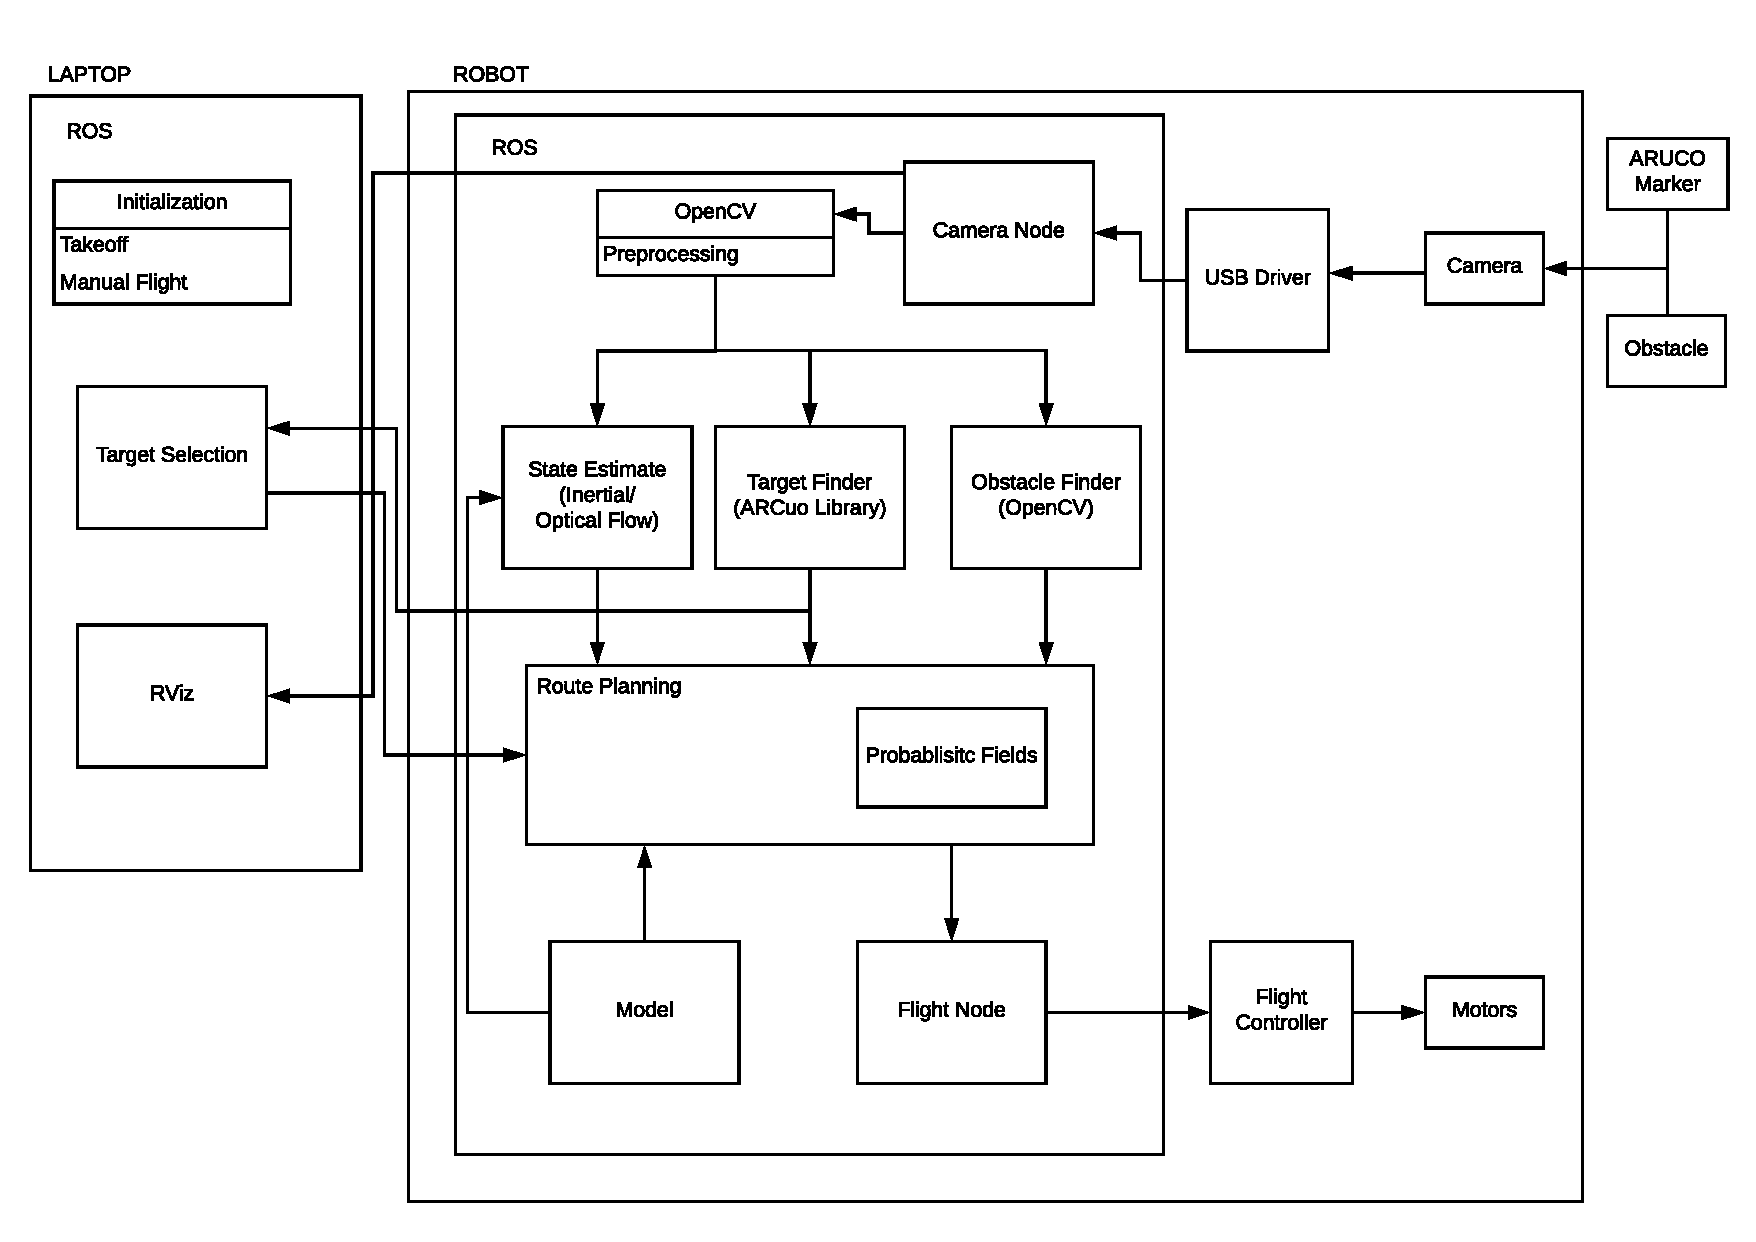
\includegraphics[width=\linewidth]{BlockDiagram}
		\caption{Project Block Diagram}
		\label{fig:blockdiagram}
	\end{figure}

	\subsection{Custom Nodes}
	
	 All of the nodes being written for this project will be written in Python and then built in ROS to be implemented on the robot. Python is being used for this project because C++ and Python are the most supported languages for both ROS Nodes and OpenCV. While C++ could possibly be faster in execution, we believe that most of our bottlenecks will be in the actual processing of images. The library calls to OpenCV will still be executing in the lower level C that OpenCV is written in, so there would be minimal gains to be had writing in C++.
	 
	 The Camera node is referenced in many locations. It is a built in node that provides image data in various formats to processes that subscribe to it, in general raw image information will be used. Common transformations that must be applied to all functions these will be done in the common camera node to avoid unnecessary calculations.
	
	\subsubsection{Target Finding}
	
	\begin{figure}[H]
		\centering
		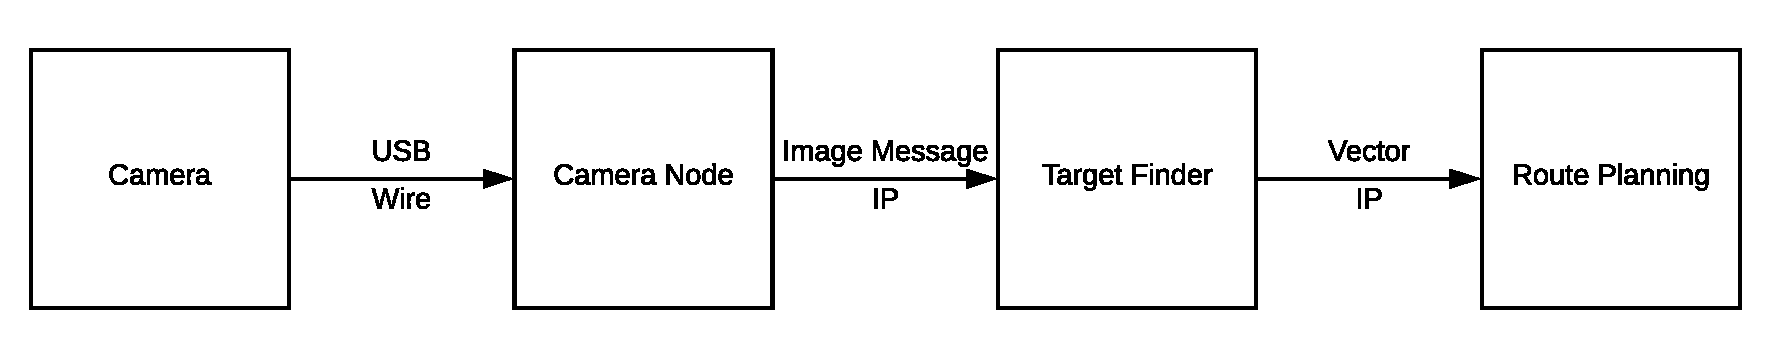
\includegraphics[width=0.9\linewidth]{Camera-Target-Route}
		\caption{Target Finding Node}
		\label{fig:target}
	\end{figure}

	Camera data, after being processed by the camera node, goes into the target finder node. The target finder is mostly implementing the ArUco symbol finding libraries in OpenCV. ArUco symbols are intended for augmented reality purposes and provide very accurate position, orientation, and distance information. These values will be translated into a vector value that the other systems on the robot can understand and be published at least 10 times per second.
	
	Given the limited field of view of the robot it may not always be able to see the target, in which case it will continue to scan for targets.
	
	ArUco markers normally encode simple ID information. Vectors will carry the same identifiers allowing the route planning parts of the robot to know when a target has been re-spotted and over-write it or allow for finding and remembering the positions of multiple targets. 
	
	\subsubsection{Obstacle Finding}
	
	\begin{figure}[H]
		\centering
		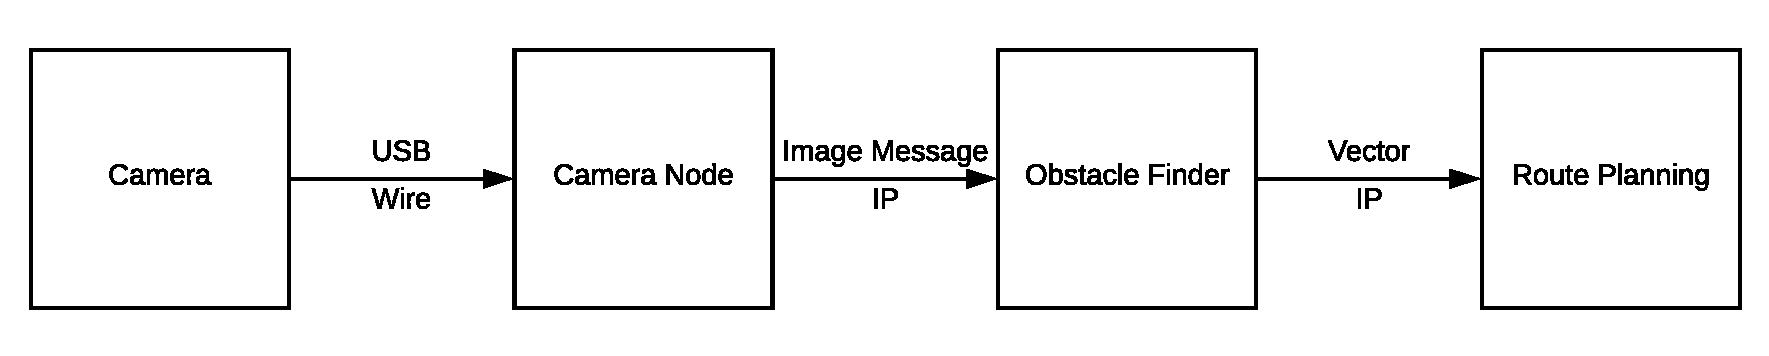
\includegraphics[width=0.9\linewidth]{Camera-Obstacle}
		\caption{Obstacle Finding Node}
		\label{fig:obstacle}
	\end{figure}

	Finding obstacles with depth information will be difficult using monocular vision. The current plan is to try to combine parallax shift with edge detection to try to parse information about nearby objects. These vectors will be published as a large ROS message at least 10 times per second. 
	
	Getting depth information from a single camera is difficuly. The TurtleBot also has a suite of depth sensors built in with the camera so these may be used initially instead of trying to use parallax information from a camera to allow for testing other aspects of the system.
	
	\subsubsection{State Estimator}
	
	\begin{figure}[H]
		\centering
		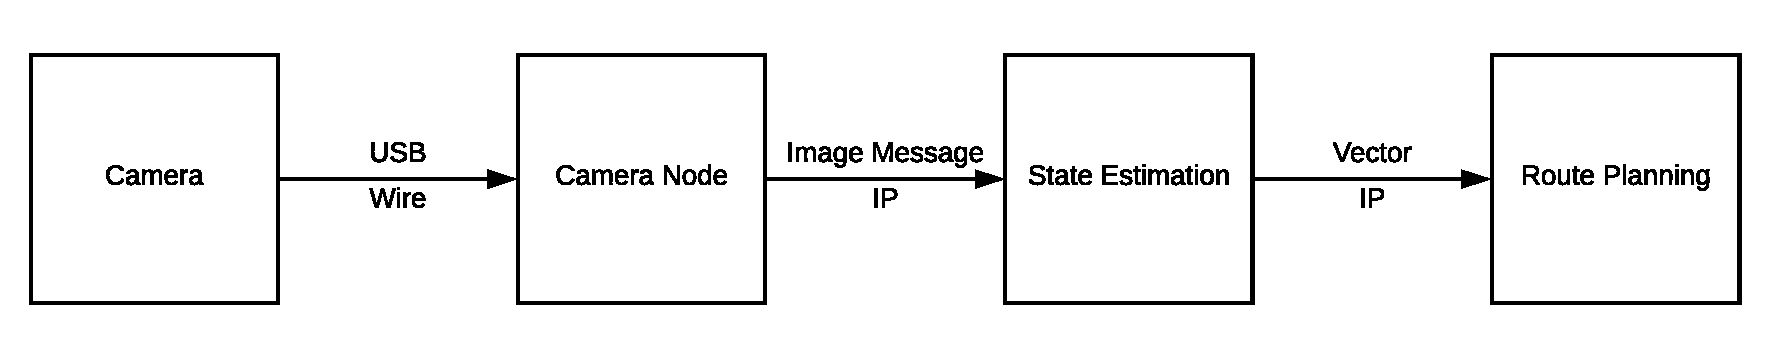
\includegraphics[width=0.9\linewidth]{Camera-State-Route}
		\caption{State Estimating Node}
		\label{fig:state}
	\end{figure}

	State estimating from camera information is very difficult and computationally expensive. The TurtleBot has stepper motors that can measure distances fairly reliably, and the Quadcopter should have accelerometers that provide changes in position more reliably than image information could. 
	
	Initially these simpler forms of measuring the robot moving through the environment will be used and transformations will be passed off to the route planning node which will adjust the vectors to nearby obstacles and targets according to how much the robot has moved. 
	
	New position estimates should be provided at least 10 times every second in the form of a transformation from the last position that the robot was in passed over a ROS message.

	\subsubsection{Route Planning}
	
	\begin{figure}[H]
		\centering
		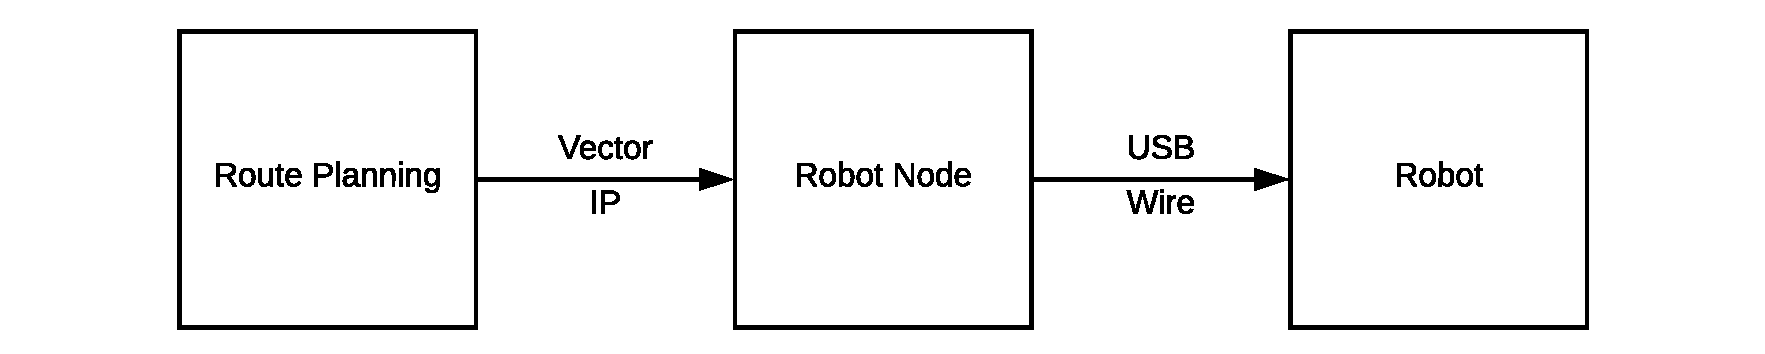
\includegraphics[width=0.9\linewidth]{Route-Planning-Robot}
		\caption{Route Planning Node}
		\label{fig:routeplanning}
	\end{figure}

	Route planning takes input from the other three custom nodes and determines a route that should carry it toward the target. The proposed solution is currently to create a potential field where positive vectors that repel the robot are attached to all obstacles while a large negative vector is attached to the target location.
	
	As the route node receives more information about the robot moving through the environment in should apply transformations to all of the contained vectors to keep them up to date with where they would be as the robot changes position in the environment. 
	
	This will also require having a method to remove un-necessary or repetitive vectors. This will be easy to implement with the target vector as the targets will have identification values meaning that the current target can be verified. With obstacles this will be more difficult, and initially vectors will probably simply expire after a certain amount of time. 
	
	The route planning software should provide a direction vector to the robot controlling node 10 times every second. There is no need for the route to be the optimal route given that the environment is unknown as we are discovering it.

	\subsection{Node Diagram}

	\begin{figure}[H]
		\centering
		\includegraphics[width=0.9\linewidth]{NodeDiagram}
		\caption{Project Node Diagram}
		\label{fig:nodediagram}
	\end{figure}


	Through Figure \ref{fig:nodediagram} it can been shown what nodes will be created or used for this project. The diagram displays what node will subscribe to the other nodes, such as the simple target finder node will subscribe to the video processor node to get messages about the target's potential location. Both the TurtleBot and the Flying Robot have two movement nodes, this is to first build a simple movement node on the platform for testing purposes, then the proper and final movement node will be made and implemented on the respective robot. 

	
	\subsection{Mathematical Modeling}
	
		\subsubsection{Flying Robot}
	
		Given that a quad-copter has six degrees of freedom, modeling them is a very difficult task. The AscTec Pelican already has many existing models indented for use with ROS. There is also a large collection of hardware agnostic tools for operating a quad-copter.
	
		\subsubsection{Robot in 3D Space}
		
		The robot itself will need to remember where it is located in its environment. Remembering where targets are located relative to the robot is necessary, and presumably remembering the locations of obstacles will be used as well. Using quaternion vectors relative to the robot will allow for simple transformations on these vectors while using very little computational power \cite{williams2010combining}. ROS contains methods and messages to easily communicate, convert, and apply transformations to quaternions.
	
		\subsubsection{Pose Estimation}
	
		Initially feedback from inertial sensors will be used for pose estimation, but ideally a version of Optical Flow would be used to estimate the position of the robot in 3D space. There are some libraries in OpenCV that have addressed generalized pose estimation in 6 degrees of freedom, but it requires a significant amount of computational power, a higher frame rate than our goal of 10Hz to be used for real time performance, and hundreds of visual odometry measurements must be made in every frame requiring a visually busy background.

	\subsection{Interfacing}
	
	The interfacing of almost all sensors with the on-board computer will be done over USB. Communication between different nodes on the same computer, and any computers off-board the robot, will be done exclusively with ROS messages sent over either internal loops or Wi-Fi.

	\subsection{Verification and Validation}
	
	\subsubsection{Unit Tests}
	
	When using ROS it is typical to create individual nodes that all execute independent of one another. Using this modular design, it is easy to write an entire node and verify it individually before executing it with the entire system.	Verification and validation of the project's nodes will be done prior to implementation in the Gazebo simulation environment.
	
	\subsubsection{Gazebo}
	
	Gazebo is a simulation environment that runs nodes that give similar input and output to nodes being executed on a real robot moving around in a real environment. This includes camera feeds, and allows for the insertion of obstacles and ArUco shapes. Testing of custom written nodes will be done in Gazebo congruently with unit-tests to ensure that nodes which rely on subscribing to other nodes are behaving as expected before executing code on an actual robot. Gazebo scheduled deadlines can be seen in Figure \ref{fig:scedulediagram}.
	
	\subsubsection{Camera Tests}
	
	Given that most of our custom nodes revolve around transforming camera data to extract information, the ArUco shapes for targets, parallax shift for obstacles, and optical flow for odometry, tests performed with only the camera and OpenCV outside of a node can be created and and executed without being contained within a ROS node. This will be useful as we can use OpenCV's feature highlighting capabilities to ensure that targets and obstacles are being identified while moving a camera through an environment. 
	
	\subsubsection{Ground Based Robot}
	
	Testing the code on a ground based robot will be necessary to ensure that the logic in the movement nodes is sound. Initially simply having the robot follow moving targets or turn to face targets that are not head on will be sufficient. As obstacle avoidance gets developed ensuring that the robot does avoid the obstacles will be enough. If the project is sufficiently developed that it is possible to fine tune the parameters of the potential fields being used by the robot to avoid obstacles and move toward an obstacle it may be necessary to use motion tracking equipment already in the lab to verify that the robot is accurately executing instructions.
	
	\subsubsection{Flying Robot}
	
	Similar to the ground based robot, verifying the flying robot will primarily involve evaluating its behaviour. The behaviour we will expect is the all the functionality that was implemented on the ground based robot previously. If more complex moves are attempted it may become necessary to test this platform using the motion capture equipment that exists in the lab.


\section{Equipment}

	\subsection{Equipment Table}
	
	A large number of items are being used in this project, most are arbitrary and may be changed in future iterations. Part way through our project we intend to re-implement the entire solution onto a different platform. A naming convention has been developed for all of our components using a three character code.
	
	The first letter, ascending from A for hardware and descending from Z for software, represents the subsystem or general classification the equipment falls under. The second character represents a generic piece of equipment, and the third is for a particular example that we are using for our project. Any part with the same two first letters should be able to be substituted freely, an example may be two cameras. One camera (CAA) may be used on the Turtlebot as it is built in to the Turtlebot frame, while another (CAB) may be used on the flying robot as it is much lighter. The generic camera (CA-) can refer to any camera which provides the same information to the same nodes.
	
	\begin{table}
		\small
		\begin{tabular}{|rl|rl|rl|}
			\hline
			\multicolumn{2}{|c|}{\textbf{Purpose}} & \multicolumn{2}{c|}{\textbf{Description}} & \multicolumn{2}{c|}{\textbf{Equipment}} \\ \hline
			A & Ground Based Robot     & A & Robot              & A   & Clearpath Robotics Turtlebot 2    \\
			A & Ground Based Robot     & B & Robot Controller   & A   & Acer Aspire E-11                  \\
			A & Ground Based Robot     & C & Robot Base         & A   & Kobuki Robot Base                 \\
			A & Ground Based Robot     & D & Sensors            & A   & Stepper Motor Feedback            \\
			A & Ground Based Robot     & D & Sensors            & B   & Orbbec Astra Pro Sensors          \\
			A & Ground Based Robot     & D & Sensors            & C   & Gyroscope                         \\ \hline
			B & Flying Robot           & A & Robot              & A   & AscTec Pelican Quadcopter         \\
			B & Flying Robot           & B & Robot Controller   & A   & AscTec Low Level Processor        \\
			B & Flying Robot           & B & Robot Controller   & B   & AscTec High Level Processor       \\
			B & Flying Robot           & B & Robot Controller   & C   & ODROID-XU4                        \\
			B & Flying Robot           & C & Robot Base         & A   & AscTec Pelican Frame              \\ \hline
			C & Camera                 & A & USB Camera         & A   & Orbbec Astra Pro Camera           \\
			C & Camera                 & A & USB Camera         & B   & oCam-1MGN-U Plus                  \\
			C & Camera                 & B & Digital Camera     & A   & AscTec Option 4                   \\ \hline
			D & Offboard Computer      & A & Computer           & A   & Lenovo T520                       \\
			D & Offboard Computer      & A & Computer           & B   & Mathworks VM - ROS Gazebo v3      \\ \hline
			E & Testing Hardware       & A & ArUco Symbol       & 0-9 & Printed Single Digit ArUco Symbol \\
			E & Testing Hardware       & B & Physical Obstacle  & A   & Human                             \\
			E & Testing Hardware       & B & Physical Obstacle  & B   & Box                               \\
			E & Testing Hardware       & B & Physical Obstacle  & C   & Sheet                             \\
			E & Testing Hardware       & C & Motion Tracking    & A   & Reflective Dot                    \\
			E & Testing Hardware       & C & Motion Tracking    & B   & Motion Tracking Cameras           \\
			E & Testing Hardware       & D & Camera Calibration & A   & Printed 7cm Checker Pattern       \\ \hline
			F & Interfacing            & A & Wireless Router    & A   & D-Link 2.4 GHz Router             \\ \hline
			S & Linux Operating System & A & Operating System   & B   & Ubuntu 18.04 Bionic               \\
			S & Linux Operating System & A & Operating System   & K   & Kubuntu (Mathworks) 14.04         \\
			S & Linux Operating System & A & Operating System   & T   & Ubuntu 14.04 Trusty               \\
			S & Linux Operating System & B & Bundled Program    & A   & Generic Loopback Device           \\
			S & Linux Operating System & C & Version Control    & A   & git                               \\ \hline
			T & ROS Service - Custom   & A & Action Services    & A   & Set Goal                          \\ \hline
			U & ROS Service - Standard & A & Action Services    & A   & Trigger                           \\ \hline
			V & ROS Message - Custom   & A & Action Messages    & A   & Goal                              \\
			V & ROS Message - Custom   & A & Action Messages    & B   & Obstacle                          \\ \hline
			W & ROS Message - Standard & A & Sensor Messages    & A   & Image                             \\
			W & ROS Message - Standard & A & Sensor Messages    & B   & PointCloud                        \\
			W & ROS Message - Standard & B & Geometry Messages  & A   & Twist                             \\
			W & ROS Message - Standard & B & Geometry Messages  & B   & Quaternion                        \\
			W & ROS Message - Standard & B & Geometry Messages  & C   & Transform                         \\ \hline
			X & ROS Node - Custom      & A & Vision             & A   & opencv\_preprocessing             \\
			X & ROS Node - Custom      & B & Movement           & A   & basic\_movement                   \\
			X & ROS Node - Custom      & B & Movement           & B   & avoidance\_movement               \\
			X & ROS Node - Custom      & B & Movement           & C   & basic\_flying\_movement           \\
			X & ROS Node - Custom      & B & Movement           & D   & avoidance\_flying\_movement       \\ \hline
			Y & ROS Node - Standard    & A & Vision             & A   & vision\_opencv                    \\
			Y & ROS Node - Standard    & A & Vision             & B   & image\_pipeline                   \\
			Y & ROS Node - Standard    & B & Coordinates        & A   & tf                                \\
			Y & ROS Node - Standard    & C & Vision             & B   & image\_pipeline                   \\ \hline
			Z & Robot Operating System & A & Operating System   & A   & ROS Indigo Igloo                  \\
			Z & Robot Operating System & A & Operating System   & B   & ROS Melodic Morenia               \\
			Z & Robot Operating System & B & Bundled Program    & A   & Gazebo2                           \\
			Z & Robot Operating System & B & Bundled Program    & B   & Gazebo7                           \\
			Z & Robot Operating System & B & Bundled Program    & C   & catkin                            \\
			Z & Robot Operating System & B & Bundled Program    & D   & RViz                              \\
			Z & Robot Operating System & B & Bundled Program    & E   & rosbag                            \\
			Z & Robot Operating System & B & Bundled Program    & F   & rqt                               \\
			Z & Robot Operating System & C & Client             & A   & roscpp                            \\
			Z & Robot Operating System & C & Client             & B   & rospy                             \\ \hline
		\end{tabular}
		\normalsize
		\caption{Equipment}
		\label{table:equipment}
	\end{table}
	
\section{Schedule}

\begin{table}[H]
	\begin{tabular}{|l|r|l|l|}
		\hline
		\multicolumn{1}{|c|}{\textbf{Task Name}}            & \multicolumn{1}{c|}{\textbf{Duration}} & \multicolumn{1}{c|}{\textbf{Start}} & \multicolumn{1}{c|}{\textbf{Finish}} \\ \hline
		\textsc{coatimunde}	            		    & \textbf{144 days} & \textbf{Tue 09/10/18} & \textbf{Sun 28/04/19} \\ \hline
		\textbf{- Turtlebot}                                & \textbf{97 days}  & \textbf{Tue 09/10/18} & \textbf{Wed 20/02/19} \\ \hline
		-- Create a Basic Movement Node                     & 12 days           & Tue 09/10/18          & Wed 24/10/18          \\ \hline
		-- Subscribe to the Camera                          & 8 days            & Wed 24/10/18          & Fri 02/11/18          \\ \hline
		\textbf{-- Camera and Video}                        & \textbf{19 days}  & \textbf{Tue 30/10/18} & \textbf{Fri 23/11/18} \\ \hline
		--- OpenCV able to process Video Stream 	    & 9 days            & Tue 30/10/18          & Fri 09/11/18          \\ \hline
		--- Able to detect a Target                         & 12 days           & Tue 08/11/18          & Fri 23/11/18          \\ \hline
		\textbf{-- Movement}                                & \textbf{67 days}  & \textbf{Tue 20/11/18} & \textbf{Wed 20/02/19} \\ \hline
		--- Move towards Target                             & 9 days            & Tue 20/11/18          & Fri 30/11/18          \\ \hline
		--- Avoid Obstacles and Move Towards Target         & 31 days           & Thu 29/11/18          & Thu 10/01/19          \\ \hline
		--- Avoid Obstacles with Memory 		    & 32 days           & Tue 08/01/19          & Wed 20/02/19          \\ \hline
		\textbf{- UAV}                                      & \textbf{53 days}  & \textbf{Wed 13/02/19} & \textbf{Sun 28/04/19} \\ \hline
		-- Port to UAV                                      & 53 days           & Wed 13/02/19          & Sun 28/04/19          \\ \hline
		\textbf{-Data Item Deliverables (DID)}		    & \textbf{148 days} & \textbf{Thu 01/11/18} & \textbf{Thu 28/03/19} \\ \hline
		-- DID-4 Preliminary Design Specification	    & 22 days		& Thu 01/11/18		& Thu 22/11/18		\\ \hline
		-- DID-5 Design Review Presentation		    & 15 days		& Thu 15/11/18		& Thu 29/11/18		\\ \hline
		-- DID-6 Schedule Update			    & 56 days		& Fri 30/11/18		& Thu 17/01/19		\\ \hline
		-- DID-7 Detailed Design Document		    & 63 days		& Fri 18/01/19		& Thu 21/03/19		\\ \hline
		-- DID-8 Final Project Presentation		    & 148 days		& Thu 01/11/18		& Thu 28/03/19		\\ \hline

	\end{tabular}
	\caption{Project Schedule}
	\label{table:projectscheduletable}
\end{table}

\begin{figure}[H]
	\centering
	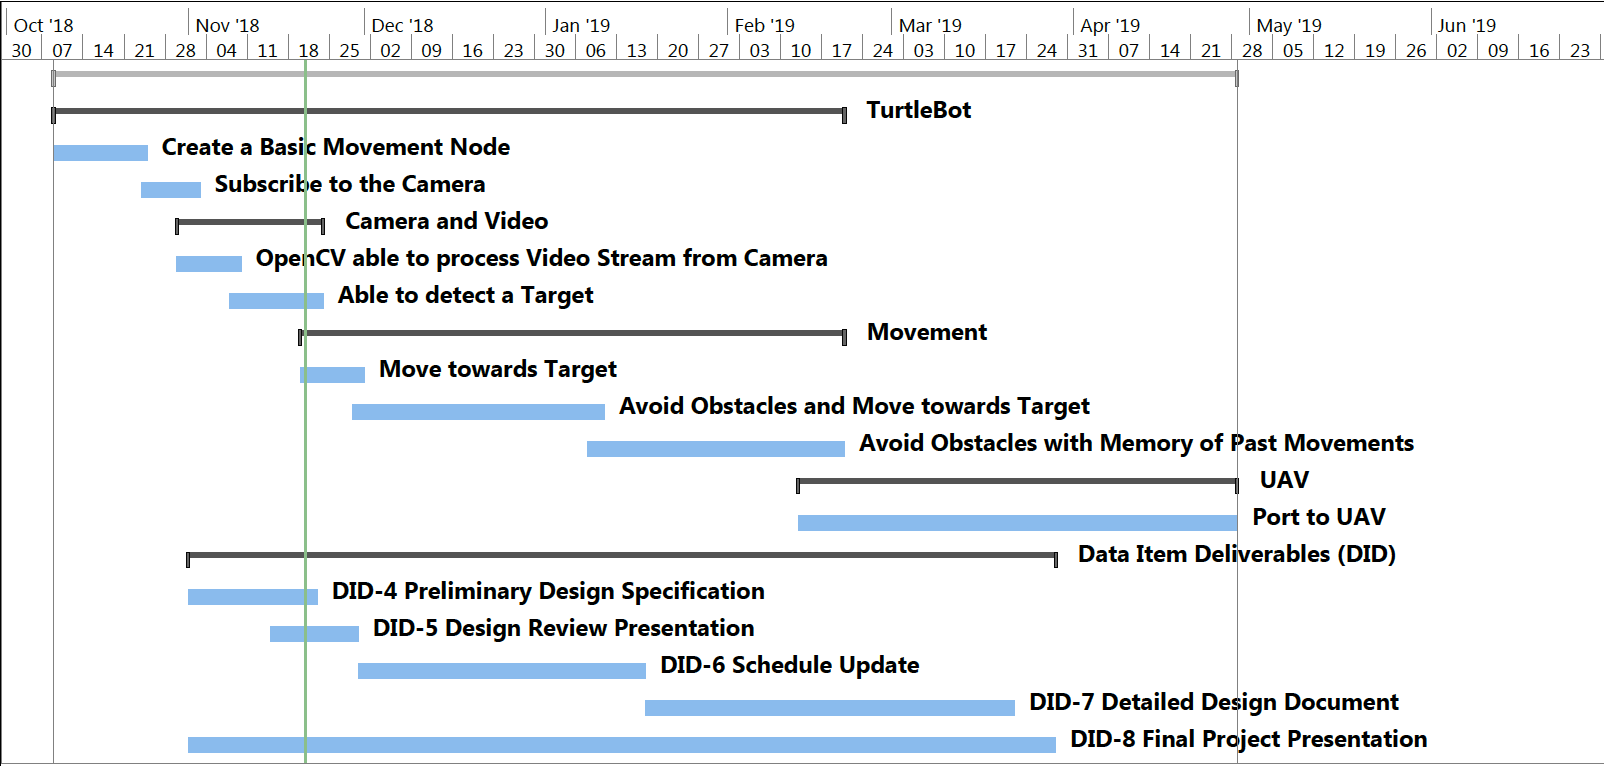
\includegraphics[width=\linewidth]{ScheduleUpdated}
	\caption{Project Schedule Diagram}
	\label{fig:schedulediagram}
\end{figure}

	The created schedule for the project shown in Fig \ref{fig:blockdiagram} outlines the major milestones for the project, such as Data Item Deliverables and deadlines for completing different functionalities for the project. Porting to the UAV is listed as one task as we aren't sure what problems will arise until we attempt to port the project.  

\section{Unresolved Issues and Risks}

	\subsection{Limited Space}
	The scope of the project is limited due to only being able to test indoors. Ideally the UAV would be operating at a high speed and identifying an arbitrary target in an unpredictable environment. In our case though the testing must be completed within the confines of a relatively small robotics laboratory. Smaller obstacles and low speeds will be used indoors due to space constraints. 

	\subsubsection{Likelihood}
	
	Guaranteed given that we are only able to test indoors without obtaining a significant number of permissions and licenses. 
	
	\subsubsection{Impact}
	
	High impact, especially if using a flying robot, as the space required simply to start and stop moving must be considered meaning limited space for obstacles.
	
	\subsubsection{Process Solution}
	
	Lower speeds will be used, and most testing will be done with a ground based vehicle. Consider requesting access to a covered sports facility during an off period of time for final testing if more space is required.
	
	\subsection{Identifying Markers}
	
	The markers we intend to use, at least initially, are intended for use in Augmented Reality purposes. Tests of these shapes show that they are capable of being identified at many angles, but the reliability with which they can be identified decreases quickly as the viewing angle changes. 
	
	There is potential that markers which are reliably identified at low speeds and in simulation may not be detectable on a flying vehicle moving faster.
	
		\subsubsection{Likelihood}
 
		Both the TurtleBot and Flying Robot shall be traveling at lower speeds, therefore the likelihood of this risk is low.
		
		\subsubsection{Impact}
		
		High impact, the primary task that our robot must accomplish is moving toward a visual target. If the robot is not able to reliably identify a marker then there will be no way to verify its capability.
		
		\subsubsection{Process Solution}
		
		Alternatives to the ArUco markers can be tested, or if these prove truly unreliable then coloured areas or illuminated targets could be incorporated. These are less desirable as ideally the robot would be able to fly toward an arbitrary target.
		
	\subsection{Computer Hardware Limitations}
	
	Image processing, especially quickly and with multiple goals, is computationally expensive. While this should not be an issue on a ground vehicle moving at slower speeds, it may become more of an issue on a Flying Robot if it operates at higher speeds and is incapable of carrying as much on-board computational capability.
	
		\subsubsection{Likelihood}

		High likelihood due to the amount of computational power required to do image processing. 
		
		\subsubsection{Impact}
		
		Medium impact, presumably we would still be able to prove our systems on the ground robot which is capable of carrying as much processing power as needed. It may also only be a limitation at higher speeds or may impose limits on what the Flying Robot is capable of identifying and tracking. 
		
		\subsubsection{Process Solution}
		
		Testing many algorithms and working to streamline the algorithm used, especially for the Flying Robot, as well as selecting hardware that is complimentary to the kind of loads created by running such an algorithm can mitigate these risks. Using an FPGA could aid with this problem.
	
	\subsection{Flight Control System Inaccuracy}
	
	Many UAV's are not able to execute arbitrary movements with high accuracy. Verifying that the flying robot is actually executing instructions may be difficult. 
	
		\subsubsection{Likelihood}
		
		Medium likelihood, depending on how well developed the libraries for our particular flying robot these issues may have all been sufficiently worked out for the purposes of this project.
		
		\subsubsection{Impact}
		
		Low impact, we could still observe the Flying Robot making decisions even if it is unable to execute the instructions given properly.
		
		\subsubsection{Process Solution}
		
		Using smaller number of obstacles and moving at a slow enough speed should ensure that the robot never needs to execute extreme moves. These more extreme moves are where inaccuracies in control models will exposes themselves the most. 


\section{Conclusion}
The preliminary design has been shown for the Flying Robot obstacle avoidance system. Background and requirement defining activities have been given to lay the groundwork and a basic understand of the current research in this domain. This document will be used and referenced for the rest of the design and building processes for the project. The design laid out in this document will also be used in the the Preliminary Design Review and Detailed Design Document. 

\printbibliography

%\end{multicols}
\end{document}    

